\documentclass[hyperref={xetex}]{beamer}
\mode<article>
{
  \usepackage{fullpage}
  \usepackage{pgf}
  \usepackage[xetex]{hyperref}
  \setjobnamebeamerversion{beamer}
}

\mode<presentation>
{
  %\usetheme{Frankfurt}
 %\usetheme{My}
  \usetheme{Madrid}
  % or ...
%\usecolortheme{seagull}
  %\setbeamercovered{transparent}
  %\setbeamercovered{dynamic}
  % or whatever (possibly just delete it)
}
\usenavigationsymbolstemplate{}
\usefonttheme{structurebold}

\setbeamertemplate{footline}
{
\leavevmode
%\hbox{\begin{beamercolorbox}[wd=.5\paperwidth,ht=2.5ex,dp=1.125ex,
%leftskip=.3cm plus1fill,rightskip=.3cm]{author in head/foot}%
%    \usebeamerfont{author in head/foot}\insertshortauthor
%  \end{beamercolorbox}%
%  \begin{beamercolorbox}[wd=.5\paperwidth,ht=2.5ex,dp=1.125ex,leftskip=.3cm,
%rightskip=.3cm plus1fil]{title in head/foot}%
%    \usebeamerfont{title in head/foot}\insertshorttitle\hfill

%\hbox{\color{gray}\insertshorttitle\hfill\insertframenumber/\inserttotalframenumber}%\hspace{3pt}}
\color{gray}\hfill\insertframenumber/\inserttotalframenumber\hspace{3pt}%
%\hspace*{2ex}
%  \end{beamercolorbox}}%
\vskip2pt%
}

\author{Jochen Schulz}
% - Use the \inst{?} command only if the authors have different
%   affiliation.

\institute{Georg-August Universit\"at G\"ottingen \pgfimage[height=0.5cm]{images/unilogo3}}
% - Use the \inst command only if there are several affiliations.
% - Keep it simple, no one is interested in your street address.

\date{}

\subject{Sage}
% This is only inserted into the PDF information catalog. Can be left
% out. 

% If you have a file called "university-logo-filename.xxx", where xxx
% is a graphic format that can be processed by latex or pdflatex,
% resp., then you can add a logo as follows:

%\logo{\pgfimage[height=0.5cm]{figures/unilogo3}}


% Delete this, if you do not want the table of contents to pop up at
% the beginning of each subsection:

\AtBeginSection[]
{
  \begin{frame}<beamer>
    \frametitle{Aufbau}
    \tableofcontents[currentsection,currentsubsection]
  \end{frame}
}

\AtBeginSubsection[]
{
  \begin{frame}<beamer>
    \frametitle{Aufbau}
    \tableofcontents[currentsection,currentsubsection]
  \end{frame}
}

\usepackage{fontspec,xunicode,xltxtra}
%\setdefaultlanguage[spelling=new, latesthyphen=true]{german}
%\setsansfont{DejaVu Sans}
%\setsansfont{Verdana}
%\setsansfont{Arial}
%\setromanfont[Mapping=tex-text]{Linux Libertine}
%\setsansfont[Mapping=tex-text]{Myriad Pro}
%\setmonofont[Mapping=tex-text]{Courier New}
%\setsansfont{Linux Biolinum}

\usepackage[ngerman]{babel}
\selectlanguage{ngerman}

%\usepackage{sagetex}

%
% math/symbols
%
\usepackage{amssymb}
% \usepackage{latexsym}
\usepackage{amsmath}
\usepackage{amsthm}
%\usepackage{amsxtra} %Weitere Extrasymbole
%\usepackage{empheq} %Gleichungen hervorheben
%\usepackage{bm}
 %\bm{A} Boldface im Mathemodus

\usepackage{multimedia}
%\usepackage{tikz}

\usepackage{cellspace}
\setlength{\cellspacetoplimit}{2pt}
\setlength{\cellspacebottomlimit}{2pt}

%%%%%%%%%%%%%%%%%% Fuer Frames [fragile]-Option verwenden!
%Programm-Listing
%%%%%%%%%%%%%%%%%%
%Listingsumgebung fuer verbatim
%Grauhinterlegeter Text
%Automatischer Zeilenumbruch ist aktiviert
\usepackage{listings}
% This command allows you to typeset syntax highlighted Matlab
% code ``inline''.
\newcommand{\isage}[1]{\lstinline|#1|}

\definecolor{lgray}{gray}{0.80}
\definecolor{gray}{gray}{0.3}
\definecolor{darkgreen}{rgb}{0,0.4,0}
\definecolor{darkblue}{rgb}{0,0,0.8}
\definecolor{key}{rgb}{0,0.5,0} 
%\lstset{backgroundcolor=\color{lgray}, frame=single, basicstyle=\ttfamily, breaklines=true}
\lstnewenvironment{sageout}[1][]{\lstset{xleftmargin=0.2cm,frame=none,backgroundcolor=\color{white},basicstyle=\color{darkblue}\ttfamily\small,#1}}{} 
\lstnewenvironment{sagein}[1][]{\lstset{#1}}{} 
%\lstnewenvironment{sage}{\lstset{,language=python, keywordstyle=color{blue},    commentstyle=color{green}, emphstyle=\color{red}, %frame=single, stringstyle=\color{red}, basicstyle=\ttfamily, ,mathescape =true,escapechar=§}}{}

%\renewcommand{\sagecommandlinetextoutput}{False}

\lstdefinestyle{SageInput}{style=DefaultSageInput,basicstyle=\ttfamily\small}
\lstdefinestyle{SageOutput}{style=DefaultSageOutput,basicstyle=\ttfamily\small}


\lstset{
language=python,
backgroundcolor=\color{lgray},
breaklines=true,
basicstyle=\ttfamily\small,
%otherkeywords={ =},
keywordstyle=\color{blue},
stringstyle=\color{darkgreen},
showstringspaces=false,
emph={class, pass, in, for, while, if, is, elif, else, not, and, or,
def, print, exec, break, continue, return},
emphstyle=\color{blue},
emph={[2]True, False, None, self},
emphstyle=[2]\color{key},
emph={[3]from, import, as},
emphstyle=[3]\color{blue},
upquote=true,
morecomment=[s]{"""}{"""},
commentstyle=\color{gray}\slshape,
%framexleftmargin=1mm, framextopmargin=1mm, 
frame=single,
mathescape =true,
escapechar=§
}


\usepackage{mydef}
%\usepackage{cmap} % you can search in the pdf for umlauts and ligatures
\usepackage{colonequals} %corrects the definition-symbols \colonequals (besides others)
\usepackage{ifthen}
%%%%%%%%%%%%%%%%%%%
%Neue Definitionen
%%%%%%%%%%%%%%%%%%%

%Newcommands
\newcommand{\Fun}[1]{\mathcal{#1}}      %Mathcal fuer Funktoren
\newcommand{\field}[1]{\mathbb{#1}}     %Grundkoerper ?? in mathds

\newcommand{\A}{\field{A}}              %Affines A
\newcommand{\Fp}{\field{F}_{\!p}}       %Endlicher Koerper mit p Elementen
\newcommand{\Fq}{\field{F}_{\!q}}       %Endlicher Koerper mit q Elementen
\newcommand{\Ga}{\field{G}_{a}}         %Add Gruppenschema
\newcommand{\K}{\field{K}}              %Generischer Koerper 
\newcommand{\N}{\field{N}}              %Nat Zahlen
\newcommand{\Pj}{\field{P}}             %Projektives P
\newcommand{\R}{\field{R}} 		%Reelle Zahlen
\newcommand{\Q}{\field{Q}}              %Rationale Zahlen  
\newcommand{\Qt}{\field{H}}             %Quaternionen 
\newcommand{\V}{\field{V}}              %Vektorbuendel V
\newcommand{\Z}{\field{Z}}              %Ganze Zahlen
\DeclareMathOperator{\Real}{Re}

\newcommand{\fdg}{\;|\;}                 %fuer die gilt

%Operatoren
\DeclareMathOperator{\Abb}{Abb}

%
% Aufgaben
%
\parindent0cm % Abs�tze nicht einr�cken 
% Definieren einer neuen Farbe
\definecolor{light-gray}{gray}{.9}

\newcounter{zaehler}     % neuen Z�hler einf�hren
\stepcounter{zaehler}    % Z�hler einen hochz�hlen

\newenvironment{aufg}[1][0]
%---- Header
{\begin{samepage}%
%\colorbox{light-gray}{%                         % Box in gray
% \makebox[\textwidth]{%                           % Box in linewidth
%\textbf{Aufgabe \arabic{zaehler} } }\hspace{-\textwidth}\makebox[\textwidth]{\hfill #1 Punkte} }\\[0.05cm]       % Header
\dotfill\\
{\large\textbf{Aufgabe \arabic{zaehler} }\ifthenelse{-1=#1}{(testierbar)}{}\ifthenelse{0=#1 \or -1=#1}{}{\hfill #1 Punkte} }\\[0.4cm]
\begin{minipage}{\textwidth}%
}%
%-----  foot
{\end{minipage}\nopagebreak%\begin{minipage}{1cm} \end{minipage}
%\\ 
%\begin{minipage}{0.1cm} \end{minipage} 
%\hrulefill \begin{minipage}{1cm} \end{minipage}\\[1cm]  
\stepcounter{zaehler}                           % increase counter
\end{samepage}%
\\%
\bigskip%
}





 
\lstset{ %
  basicstyle=\tiny,           % the size of the fonts that are used for the code
  numbers=left,                   % where to put the line-numbers
  numberstyle=\tiny\color{gray},  % the style that is used for the line-numbers
  stepnumber=1,                   % the step between two line-numbers. If it's 1, each line 
                                  % will be numbered
  numbersep=5pt,                  % how far the line-numbers are from the code
  backgroundcolor=\color{white},      % choose the background color. You must add \usepackage{color}
  showspaces=false,               % show spaces adding particular underscores
  showstringspaces=false,         % underline spaces within strings
  showtabs=false,                 % show tabs within strings adding particular underscores
  frame=single,                   % adds a frame around the code
  rulecolor=\color{black},        % if not set, the frame-color may be changed on line-breaks within not-black text (e.g. commens (green here))
  tabsize=2,                      % sets default tabsize to 2 spaces
  captionpos=b,                   % sets the caption-position to bottom
  breaklines=true,                % sets automatic line breaking
  breakatwhitespace=false,        % sets if automatic breaks should only happen at whitespace
  title=\lstname,                   % show the filename of files included with \lstinputlisting;
                                  % also try caption instead of title
  keywordstyle=\color{blue},          % keyword style
  commentstyle=\color{gray},       % comment style
  stringstyle=\color{mauve},         % string literal style
  escapeinside={\%*}{*)},            % if you want to add LaTeX within your code
  morekeywords={*,...}               % if you want to add more keywords to the set
}

\title{Das Praxis-Problem von remote Filesystemen in der NAM}
\subtitle{ Ceph, DiscoFS, ZFS, Client-Sync, \ldots}
\author{Jochen Schulz, Ralph Krimmel, Max Voit}



\begin{document}
	\nocite{*} 
	\begin{frame}
		\titlepage
	\end{frame}

	\begin{frame}
		\tableofcontents
	\end{frame}


\section{Einf\"uhrung und Motivation}
\subsection*{}

\begin{frame}{Philosophie und gewünschtes Setup}
    \begin{block}{A: Synchron}
    \begin{itemize}    
        \item Compute-server: (Fokus: Compute)
        \item Clients: Laptops mit remote gemounteten Home (Fokus: tägliche Arbeit)
        \item (File-)Server: (Fokus: shared ressources)
    \end{itemize}
\end{block}

\begin{block}{B: Asynchron}
    \begin{itemize}
                    \item  Daten stets (auch) lokal. 
                    \item Asynchroner Datenabgleich mit remote storage (dropbox,powerfolder,git \ldots )
                \end{itemize}

\end{block}
\end{frame}

\begin{frame}{Philosophie und gewünschtes Setup}

\begin{block}{Prinzipielle Vor- und Nachteile}
    \begin{itemize}
        \item A: Flexibilität im Ort und Gerät (Keine Transferzeit)
        \item A: Parallelität
        \item A: Homogenität und Synchrones Arbeiten (z.B. lokales Editieren , remote Ausführen)
        \item B: Mobilität des Geräts
        \item B: Daten stets lokal (aber Transferzeit)
    \end{itemize}
    
\end{block}
    

\end{frame}


\begin{frame}{Details bestehendes Setup (Typ A)}
	\begin{itemize}
        \item \alert{clients ($\approx$ 50):} Linux-Laptops, Datensync per unison
        \item \alert{Login Server (2):} remote Desktop, ssh, Datentransfer
        \item \alert{Compute Server (6):} remote Desktop, ssh, Datentransfer, FHGFS, WiRe, CUDA
        \item \alert{Fileserver (2):} (kein SAN)
			\begin{itemize}
				\item lokales Dateisystem: ZFS 
				\item Netzwerkdateisystem: NFS (v3) und samba
                \item \textsl{Hot spare Replikation} durch AVS
			\end{itemize} 
        \item <2> \alert{Sonstige Server (6):} Virtualisiert mit OpenVZ
	\begin{itemize}
		\item Email \& Groupware und LDAP
		\item Diverse Lizenzserver
		\item Nameserver und dhcpd
        \item puppet und FAI    
	\end{itemize}
	\end{itemize}
\end{frame}

\begin{frame}{Schwierigkeiten des Setups}

	\begin{itemize}
		\item Fileserver
			\begin{itemize}
				\item ZFS  (nur lokal)
				\item NFS hat nur einen Zugangsknoten$\Rightarrow$ ineffiziente Hardware-Nutzung, keine intrinsische Redundanz
                \item NFS wegen Sicherheit und des clientssetups nur intern nutzbar
                \item \textbf{AVS} verursacht Last auf dem Haupt-Server
            \end{itemize} 
		\item <2-3> Sonstige Server
			\begin{itemize}
				\item Unbenutzte Speicherkapazit\"at
				\item Unbenutzte Rechenkapazit\"at (Balancing nur schwer möglich)
				\item Unzureichende Verf\"ugbarkeit bei Fehlern (single point of failure)
			\end{itemize}
        \item <3> Clients
             \begin{itemize}
                 \item Nicht sehr mobil (Mobilität erfordert Restart)
                 \item Datensynchronisation (Unison) kostet Zeit und Ressourcen bei Login/Logout
                 \item User muss Vorgang verstehen und beobachten.
			\end{itemize}
	\end{itemize}
\end{frame}


\begin{frame}{Verbesserungsansatz - Serverseitig}
		Nutzung von verteilten, fehler-toleranten Dateisystem (Distributed parallel fault-tolerant file systems) und damit storage-cluster und VM-Cluster.


	%		\begin{itemize}
	%			\item Ausfalltoleranz (Verf\"ugbarkeit und Zuverl\"assigkeit) durch Replikation
	%			\item Hohe Performanz durch Striping %Aufteilen der Daten auf mehrere physikalische Devices
	%		\end{itemize}
	
    \begin{block}{Varianten}
        Hinweis: Grossteils alte Hardware ohne HVM/SVM-Flag
	\begin{itemize}
		\item [$\alpha$]Jeder Server wird gleichzeitig Hypervisor und Storage-Knoten. 
            \begin{itemize}
                \item  LXC + Ceph (fuse)
                \item  LXC + Glusterfs (fuse)
                \item  OpenVZ + Lustre (alter Kernel!)
            \end{itemize}
        \item [$\beta$] Storage-Cluster getrennt vom VM-Cluster.
            \begin{itemize}
                \item OpenVZ + Ceph (getrennt wegen inkompatibler Kernel-Version)
                \item Xen + Ceph RBD (getrennt wegen RBD kernel Treiber)
                \item LXC + CephFS  (getrennt wegen kernel Treiber)
            \end{itemize}
	\end{itemize}
        
    \end{block}

\end{frame}

\begin{frame}{Verbesserungsansatz - Clientseitig}
    \begin{itemize}
        \item Home abkoppeln, nur einzelne Verzeichnisse mounten. 
        \item DiscoFS . FS-Overlay mit vollständigen lokalen Cache (FUSE)
        \item Ceph-erweiterung für disconnected operations
    \end{itemize}
\end{frame}

\begin{frame}{DiscoFS - DISCOnnected File System}
(Von Robin Martinjak) \href{DiscoFS}{https://github.com/rmartinjak/discofs}
\begin{block}{Idee}
FS-Overlay über lokalen Daten und remote Daten, die in Sync gehalten werden sollen.
\end{block}
\begin{itemize}
    \item disconnected operations: Bei disconnect lokal, bei connect lokal und remote. 
    \item Conflict-Handling wenn sich beide Quellen geändert haben.
\end{itemize}

Komponenten: 
\begin{itemize}
    \item Cache: lokale Daten
    \item Sync table: Synctime of file objects
    \item Job: Replikation organisieren
    \item Database: Job und Sync-Daten speichern
    \item State check Thread: Online-Status prüfen.
    \item worker Thread: Jobs abarbeiten
\end{itemize}

\end{frame}

\begin{frame}{Ceph-Erweiterung}
    \begin{block}{Idee}
Benutze CRUSH um eine zusätzliche Replica eines Homes lokal auf dem Laptop abzulegen.        
    \end{block}
    \begin{itemize}
        \item Geht die Verbindung verloren sind alle Daten lokal und, theoretisch, kann der lokale Ceph-clientweiterarbeiten.
        \item Das Wiederverbinden ists bereits implementiert, allerdings bräuchte man noch ein Conflict-Handling.
    \end{itemize}


%potentially taking a crack at ceph-deploy
%(https://github.com/ceph/ceph-deploy) in the meantime as that may be a
%key piece of how you can roll out various pieces if it becomes more
%robust.

%Patrick told me briefly about the disconnected laptop idea.  My initial 
%reaction is that this is a hard problem, but that there are some elements 
%in the Ceph MDS that could make this work better than in other systems.  
%%My assumption would be that you'd only want certain directories to be 
%mirrored onto the mobile system, and that you'd allow divergent 
%modifications, and resolve conflicts later.  The MDS's recursive mtime 
%stuff would be one tool that would enable efficient recovery.  It may also 
%be possible to build in a sort of 'op log' into the MDS for specific 
%directories to enable an efficient sync (and handle things like directory 
%rename efficiently).  I'm not sure that piggybacking on the DR framework 
%would be the way to go.  All in all, though, a very interesting direction 
%to go in, and something that would be great to look at.

%That said, it's not something we (Inktank) would be able to work on 
%directly, as we have other pressing priorities.  We can certainly work 
%with you with design issues and with navigating the MDS code of course.

%Anyway, that all said, if you are looking for something simpler to start 
%with, there are lots of areas where some outside (devops) expertise can be 
%applied.  There is going to be some management API work (a REST gateway 
%and API to supplement the current CLI).  There's also ceph-deploy, which 
%is an interesting prototype at this stage but needs lots of work (Linux 
%distro independence, uninstall, etc.).
\end{frame}

\subsection{Ausflug ZFS}

%\begin{frame}{Definition}
%		In computing, a distributed file system or network file system is any file system that allows access to files from multiple hosts via a computer network.$[1]$
%	\tiny{$[1]$ Galvin Silberschatz (1994). Operating System concepts, chapter 17 Distributed file systems. Addison-Wesley Publishing Company.} \\ 
%\end{frame}

\begin{frame}{ZFS - die eierlegende Wollmilchsau der lokalen Filesysteme}
    Betriebssystem : Nexenta (Ubuntu mit einem Opensolaris-Kernel)\\
    ZFS Eckdaten:
    \begin{itemize}
        \item virtuelle Partitionen: zpool (lvm)
        \item eingebautes Redundanz RAID (dmraid). RaidZ
        \item Snapshots, Encyption, Compression
        \item Copy-on-Write
        \item Sharing (nfs, samba)
        \item \ldots
    \end{itemize}
    \alert{Praxis:} (Fast) alle Erwartungen wurden erfüllt. \\
    \begin{itemize}
        \item NFSv4 (war) instabil (aber eigentlich kein ZFS-Problem)
        \item Komplexität kommt mit Intransparenz. 
        \item Abstürze, Filesystem-Hänger, Snapshot-Performance
        \item Benchmark
    \end{itemize}
\end{frame}

\begin{frame}{Fileserver Availability durch AVS}
    Blockbasiert, weiss nichts von ZFS.
	\begin{center}
	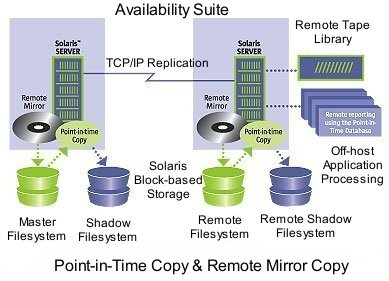
\includegraphics[width=0.65\textwidth]{images/availabilitysuitenew.jpg}
	\end{center}
	\small
	Quelle: \texttt{http://hub.opensolaris.org/bin/view/Project+avs/}
\end{frame}

\section{Parallel, distributed, fault-tolerant filesystems}
\begin{frame}{Anforderungen an ein verteiltes Dateisystem}
	\begin{itemize}
		\item Hohe Performanz durch Striping
			\begin{itemize}
				\item Durchsatz
				\item Latenz
			\end{itemize}
		\item Skalierbarkeit
		\item Verf\"ugbarkeit
		\item Zuverl\"assigkeit
	\end{itemize}
\end{frame}

\begin{frame}{Zuverl\"assigkeit/Verf\"ugbarkeit}
	Problem: Fehler sind mehr die Norm als die Ausnahme
	\begin{itemize}
		\item System g\"unstiger Hardware
		\item Fehler in Programmen %theres software that always crashes 
		\item Menschliches Versagen % what was this cable for?
		\item Betriebssystemfehler % ever used windows?
		\item Ausfall von: 
		\begin{itemize}
			\item Festplatten
			\item Arbeitsspeicher
			\item Kabel
			\item Netzwerk
			\item ...
		\end{itemize}
	\end{itemize}		
\end{frame}

\begin{frame}{Moderner Ansatz}
	\begin{itemize}
		\item Objektbasiert
		\item Festplatten $\rightarrow$ Intelligent object storage devices (OSD's)
		\begin{itemize}
			\item CPU
			\item Netzwerkschnittstelle
			\item Lokaler Cache
		\end{itemize}
		\item Metadaten getrennt von Nutzdaten
	\end{itemize}
\end{frame}


\begin{frame}{Typischer Zugriff (z.B. Hadoop)}
	\begin{center}
	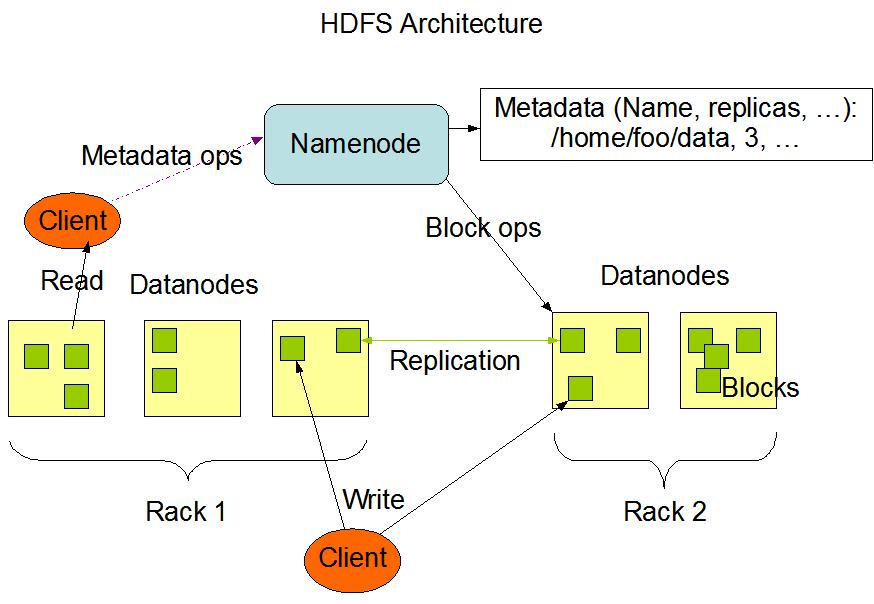
\includegraphics[scale=0.2]{images/hdfsarchitecture.jpg}
	\end{center}
	\small
	Quelle: \texttt{http://hadoop.apache.org/common/docs/r0.20.2/hdfs\_design.html}
\end{frame}

\subsection{Auswahl verteilte Dateisysteme}
\begin{frame}{Auswahl verteilte Dateisysteme}
	\begin{description}	
        \item [Lustre]  Alter Kernel und nur ein Metadatenserver \\
        \item [Google FS] Propriet\"ar, ausgelegt auf große Dateien \\
        \item [GlusterFS]  Nur FUSE, keine advanced features; im Vergleich Langsam (siehe Benchmark)\\
        \item [XtremeFS] nett ;) aber Fokus liegt auf Geo-Features\\
        \item [FHGS]  Propriet\"arer server, Opensource client. keine Redundanz, im HPC-Umfeld aber gut (Bei uns seit kurzem im Einsatz).
        \item [pNFS] Vielversprechend, bisher aber keine Tests durchgeführt (zu spät?)
	\end{description}
\end{frame}

\subsection{Ceph Theorie}

\begin{frame}{Ceph - \"Ubersicht}
	
	Drei Komponenten:
	\begin{itemize}
        \item \alert{Client:} Posix\"ahnliche Schnittstelle %Stellt zur verfuegung
        \item \alert{OSD Cluster:} Speichert Daten und Metadaten
        \item \alert{Metadaten Cluster}
			\begin{itemize}
				\item Verwaltet Namensraum
				\item Konsistenz/Koh\"arenz
				\item Sicherheit (Noch nicht ausreichend implementiert)
			\end{itemize}
	\end{itemize}
\end{frame}

\begin{frame}
	\begin{center}
		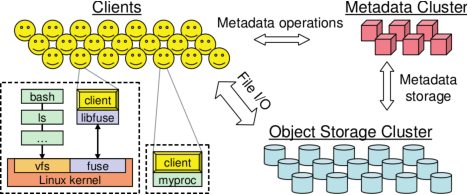
\includegraphics{images/ceph_architecture.pdf}
	\end{center}
    Quelle: \cite{weil_ceph:_2006}
\end{frame}


\begin{frame}{Design Features}
	\begin{itemize}
		\item Trennung der Verwaltung von Daten und Metadaten
		\begin{itemize}
			\item Unabhaengige Skalierbarkeit
			\item Keine Block/Objektlisten (CRUSH)
		\end{itemize}
		\item  Dynamische Verteilung der Metadaten
		\begin{itemize}
			\item Halber Aufwand sind Metadatenoperationen
			\item Gutes Loadbalancing der Metadaten ist \"außerst wichtig %fuer performance
		\end{itemize}
		\item Autonomes OSD Cluster verantwortlich f\"ur:
			\begin{itemize}
				\item Replikation
				\item Fehlererkennung
				\item Wiederherstellung nach Fehlern
			\end{itemize}
	\end{itemize}	
\end{frame}

\begin{frame}{Dateizugriff}

\begin{enumerate}
	\item Client sendet Dateirequest an das MDS Cluster
	\item Ein MDS \"ubersetzt Dateiname in \textit{file inode}
	\begin{itemize}
		\item Unique inode number
		\item Besitzer
		\item Gr\"oße
		\item ...
	\end{itemize}
	\item MDS gibt inode number, Gr\"oße und Verteilungsstrategie zur\"uck
	\item Direkter Zugriff von Client auf OSD
\end{enumerate}
\end{frame}

\begin{frame}{Dynamische Metadaten-Verteilung}
	\begin{center}
		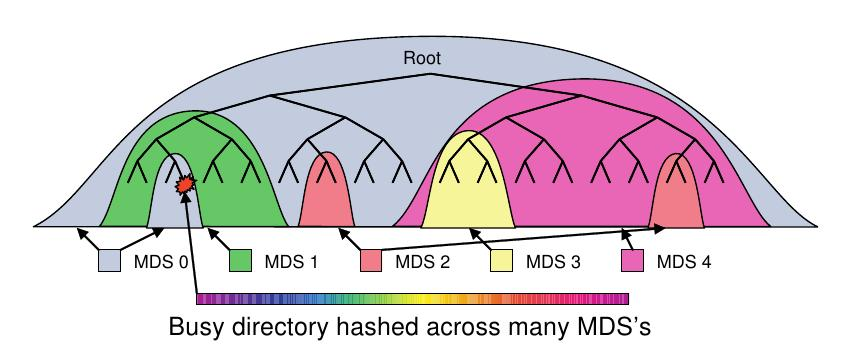
\includegraphics[width=0.8\textwidth]{images/mds.jpg}
	\end{center}
    Quelle: \cite{weil_ceph:_2006}
\end{frame}

\begin{frame}{Client Synchronisierung}
	Problem: Mehrere Clients schreiben/lesen eine Datei gleichzeitig.

	\begin{itemize}	
		\item Kein read caching/write buffering mehr
		\item I/O der clients synchron %blocked until acked
			\begin{itemize}
				\item Synchrone I/O schlecht f\"ur Client Performanz
			\end{itemize}
		\item HPC Erweiterung: O\_LAZY flag f\"ur \texttt{open}
	\end{itemize}
\end{frame}


\begin{frame}{CRUSH}
	\begin{center}
	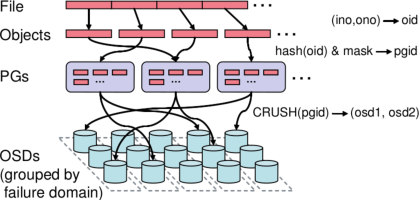
\includegraphics{images/crush.pdf}
\end{center}
\end{frame}

\begin{frame}{CRUSH!}
%    \begin{center}
%    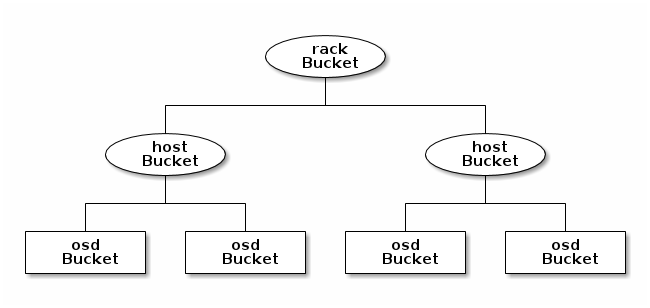
\includegraphics[width=0.8\textwidth]{images/crush.png}
%\end{center}

Für $x \in \mathbb{N}$ ist $CRUSH$ eine Abbildung nach $R \in \mathbb{N}^n$ für $n  \in \mathbb{N}$.

$x$ : Data-Object\\
$R$ : Placement für $n$ Replicas
 
\end{frame}

\subsection{Ceph Praxis}


\begin{frame}{Vorraussetzungen}
	\begin{itemize}
		\item Ausgeschaltetes Write Caching auf der Festplatte
		\item Dateisystem mit \emph{Extended Attributes (XATTRs)}:
		\begin{itemize}
			\item XFS
			\item BTRFS
%			\item Internet Status der Objekte
%			\item Snapshot Metadaten
%			\item RADOS Gateway Access Control Lists (ACLs).
		\end{itemize}
		\item Empfohlen: Disk je OSD

	\end{itemize}
\end{frame}



\begin{frame}{Installation}

	Einfach, Pakete vorhanden f\"ur:
	\begin{itemize}
		\item Ubuntu
		\begin{itemize}
			\item natty
			\item oneiric
			\item precise
		\end{itemize}
		\item Debian
		\begin{itemize}
			\item sid
			\item squeeze
			\item wheezy
		\end{itemize}
		\item RPM 
		\begin{itemize}
			\item Selbst bauen per \texttt{rpmbuild}
		\end{itemize}
	\end{itemize}

\end{frame}


\begin{frame}{Cluster Design}
	3 Daemons
	\begin{itemize}
        \item \alert{ceph-osd}: Object Storage
        \item \alert{ceph-mds}: Metadaten Server: Verteilter, koh\"arenter Cache f\"ur Metadaten %agiert
        \item \alert{ceph-mon}: Monitor, Cluster Management, Konfiguration und Zugangspunkt f\"ur CephFS
	\end{itemize}
\end{frame}


\begin{frame}{Object Storage Daemon}
	\begin{itemize}
		\item Mehrere OSDs pro Host m\"oglich
		\item Hardware Vor.:
		\begin{itemize}
			\item Viele Festplatten 
			\item Viel Ram (besseres Caching) (min. 500MB/Daemon)
			\item Schnelles Netzwerk
		\end{itemize}
		\item Anzahl:
		\begin{itemize}
			\item Mindestens 2, so viele wie m\"oglich
		\end{itemize}
	\end{itemize}
\end{frame}


\begin{frame}{Metadaten Daemon}
	\begin{itemize}

		\item Hardware Vor.:
		\begin{itemize}
			\item Sehr viel Ram
			\item Schnelle CPU
			\item Schnelles Netzwerk (geringe Verz\"ogerung)
		\end{itemize}
		\item Anzahl: 
		\begin{itemize}
			\item Mindestens 1
			\item 2 oder mehr f\"ur Redundanz und Load Balancing
		\end{itemize}
	\end{itemize}
\end{frame}


\begin{frame}{Monitor Daemon}
	\begin{itemize}
		\item Hardware Vor.:
		\begin{itemize}
			\item Einige GB Festplattenspeicher
			\item Feste IP
		\end{itemize}
		\item Anzahl:
		\begin{itemize}
			\item Ungerade Anzahl!
			\item 1 ist ok
			\item 3 ideal f\"ur die meisten Anwendungsf\"alle
			\item Mehr nur f\"ur sehr große Cluster
		\end{itemize}
	\end{itemize}
\end{frame}

\begin{frame}[fragile]{Beispiel ceph.conf}

\begin{lstlisting}
;This is a comment
[global]
	auth supported = cephx
[osd]
	osd journal size = 1000
[mon.a]
	host = myserver01
	mon addr = 10.0.0.101:6789
[mon.b]
	host = myserver02
	mon addr = 10.0.0.102:6789
[mon.c]
	host = myserver03
	mon addr = 10.0.0.103:6789
[osd.0]
	host = myserver01
[osd.1]
	host = myserver02
[osd.2]
	host = myserver03
[mds.a]
	host = myserver01
\end{lstlisting}
\end{frame}



\begin{frame}{Deployment}
	\begin{itemize}
		\item Chef cloud management tool (nicht getestet)
		\item \textbf{mkcephfs} (f\"ur Testzwecke)
			\begin{enumerate}
				\item Ben\"otigt passwortlosen \texttt{root}-Login auf allen Hosts
				\item Kopieren der ceph.conf auf alle Hosts
				\item Erstellen der Standardordner z.B. f\"ur myserver03
				\begin{description}
					\item \texttt{mkdir /var/lib/ceph/osd/ceph-2}
					\item \texttt{mkdir /var/lib/ceph/mon/ceph-c}
				\end{description}
				\item \texttt{mkcephfs -a -c /etc/ceph/ceph.conf -k /etc/ceph/ceph.keyring}
			\end{enumerate}
	\end{itemize}
\end{frame}


\begin{frame}[fragile]{CRUSH-map}
    \begin{lstlisting}
# buckets
host paimutan {
        id -2           # do not change unnecessarily
        # weight 1.000
        alg straw
        hash 0  # rjenkins1
        item osd.0 weight 1.000
}
host darjeeling {
        id -4           # do not change unnecessarily
        # weight 1.000
        alg straw
        hash 0  # rjenkins1
        item osd.1 weight 1.000
}
rack unknownrack {
        id -3           # do not change unnecessarily
        # weight 6.000
        alg straw
        hash 0  # rjenkins1
        item paimutan weight 1.000
        item darjeeling weight 1.000
        item gunpowder weight 1.000
        item earlgrey weight 1.000
        item lemongrass weight 1.000
        item oolong weight 1.000
}
pool default {
        id -1           # do not change unnecessarily
        # weight 6.000
        alg straw
        hash 0  # rjenkins1
        item unknownrack weight 6.000
}
    \end{lstlisting}
\end{frame}

\begin{frame}{Zugriff}
	\begin{itemize}
		\item Kerneltreiber
		\item FUSE
		\item librados (RBD)
		\item Rados Gateway (RESTful interface)
	\end{itemize}
\end{frame}

\section{Erfahrungen}

\begin{frame}{CephFS}
    \begin{block}{Gut}
        Selbstheilung sehr gut.
    \end{block}
    %nur bei extremen Ausfaellen und Netz-beintraechtigung ging der Cluster in die Knie (degraded).
    %Nur einmal bei so einem Test gab es permanenten Datenverlust und wir mussten den cluster neu formatieren.
    \begin{block}{Schlecht}
    \begin{itemize}
        \item Crash bei mount mit dem Kernel Treiber auf OSD-Server (per Design).
        \item Performance bei vielen kleinen Dateien/Datenbanken noch relativ gering (Hardware?).
    \end{itemize}
\end{block}
\end{frame}

\begin{frame}{bisherige Benchmarks}
Benchmark: \url{https://rcs.num.math.uni-goettingen.de/virt-benchmark/composite.xml}

\end{frame}
\begin{frame}{Zusammenfassung}
\begin{itemize}
	\item Sehr vielversprechend und in aktiver Entwicklung.
\item Team sehr offen und hilfsbereit
	\item Einiges unvollst\"andig implementiert (Sicherheit)
\end{itemize}
	\begin{center}
	\large Fragen? Anregungen? Vorschl\"age? 
	\end{center}
\end{frame}

	

\begin{frame}{Literatur}
	\bibliographystyle{apalike}
	\bibliography{ceph}	
\end{frame}

\end{document}


